% THIS IS SIGPROC-SP.TEX - VERSION 3.1
% WORKS WITH V3.2SP OF ACM_PROC_ARTICLE-SP.CLS
% APRIL 2009
%
% It is an example file showing how to use the 'acm_proc_article-sp.cls' V3.2SP
% LaTeX2e document class file for Conference Proceedings submissions.
% ----------------------------------------------------------------------------------------------------------------
% This .tex file (and associated .cls V3.2SP) *DOES NOT* produce:
%       1) The Permission Statement
%       2) The Conference (location) Info information
%       3) The Copyright Line with ACM data
%       4) Page numbering
% ---------------------------------------------------------------------------------------------------------------
% It is an example which *does* use the .bib file (from which the .bbl file
% is produced).
% REMEMBER HOWEVER: After having produced the .bbl file,
% and prior to final submission,
% you need to 'insert'  your .bbl file into your source .tex file so as to provide
% ONE 'self-contained' source file.
%
% Questions regarding SIGS should be sent to
% Adrienne Griscti ---> griscti@acm.org
%
% Questions/suggestions regarding the guidelines, .tex and .cls files, etc. to
% Gerald Murray ---> murray@hq.acm.org
%
% For tracking purposes - this is V3.1SP - APRIL 2009

%\documentclass{acm_proc_article-sp}
\documentclass{sig-alternate}
\usepackage[numbers, sort, compress]{natbib}
\usepackage{graphics}
\usepackage{graphicx}
\usepackage{epstopdf}
\usepackage{color}
\usepackage{hyperref}
\usepackage{pdfsync}
\usepackage{mdwlist}

\begin{document}

\conferenceinfo{ECMLS'12,} {}
\CopyrightYear{2012}
\crdata{978-1-4503-0702-4/11/06}
\clubpenalty=10000
\widowpenalty = 10000


%\title{A Sample {\ttlit ACM} SIG Proceedings Paper in LaTeX
%Format\titlenote{(Does NOT produce the permission block, copyright information nor page numbering). For use with ACM\_PROC\_ARTICLE-SP.CLS. Supported by ACM.}}

\newif\ifdraft
%\drafttrue                                                                                                   

\ifdraft
% \newcommand{\reviewer}[1]{ {\textcolor{blue}    { ***Reviewer:     #1 }}}
 \newcommand{\jkimnote}[1]{{\textcolor{green}   { ***Joohyun:   #1 }}}
 \newcommand{\jhanote}[1]{  {\textcolor{red}     { ***SJ: #1 }}}
  \newcommand{\pmnote}[1]{  {\textcolor{red}     { ***Pradeep: #1 }}}
 \newcommand{\todo}[1]{  {\textcolor{red}     { ***TODO: #1 }}}
 \newcommand{\fix}[1]{  {\textcolor{red}     { ***FIX: #1 }}}
 \newcommand{\reviewer}[1]{}
\else
 \newcommand{\reviewer}[1]{}
 \newcommand{\jkimnote}[1]{}
 \newcommand{\pmnote}[1]{}
 \newcommand{\jhanote}[1]{}
 \newcommand{\todo}[1]{  {\textcolor{red}     { ***TODO: #1 }}}
 \newcommand{\fix}[1]{}                                                                                     
\fi

\title{Next-Generation Sequencing Reads Alignment using SAGA-MapReduce}

\numberofauthors{3} %  in this sample file, there are a *total*
% of EIGHT authors. SIX appear on the 'first-page' (for formatting
% reasons) and the remaining two appear in the \additionalauthors section.
%
\author{
% You can go ahead and credit any number of authors here,
% e.g. one 'row of three' or two rows (consisting of one row of three
% and a second row of one, two or three).
%
% The command \alignauthor (no curly braces needed) should
% precede each author name, affiliation/snail-mail address and
% e-mail address. Additionally, tag each line of
% affiliation/address with \affaddr, and tag the
% e-mail address with \email.
%
\alignauthor Pradeep Kumar Mantha\\
       \affaddr{Center for Computation and Technology}\\
       \affaddr{Louisiana State University}\\
       \affaddr{216 Johnston}\\
       \affaddr{Baton Rouge, LA}
       \email{pradeepm66@gmail.com}
\alignauthor Andre Luckow\\
       \affaddr{Center for Computation and Technology}\\
       \affaddr{Louisiana State University}\\
       \affaddr{216 Johnston}\\
       \affaddr{Baton Rouge, LA}
       \email{yours are here}       
\alignauthor Joohyun Kim\titlenote{Author for correspondence}\\
       \affaddr{Center for Computation and Technology}\\
       \affaddr{Louisiana State University}\\
       \affaddr{216 Johnston}\\
       \affaddr{Baton Rouge, LA} \\
       \email{jhkim@cct.lsu.edu}
\alignauthor Shantenu Jha\titlenote{Author for correspondence}\\
      \affaddr{Center for Computation and Technology}\\
     \affaddr{Louisiana State University}\\
      \affaddr{214 Johnston}\\
      \affaddr{Baton Rouge, LA}
     \email{sjha@cct.lsu.edu}
}
% There's nothing stopping you putting the seventh, eighth, etc.
% author on the opening page (as the 'third row') but we ask,
% for aesthetic reasons that you place these 'additional authors'
% in the \additional authors block, viz.
%\additionalauthors{Additional authors: John Smith (The Th{\o}rv{\"a}ld Group,
%email: {\texttt{jsmith@affiliation.org}}) and Julius P.~Kumquat
%(The Kumquat Consortium, email: {\texttt{jpkumquat@consortium.net}}).}
\date{25 Feb. 2012}
% Just remember to make sure that the TOTAL number of authors
% is the number that will appear on the first page PLUS the
% number that will appear in the \additionalauthors section.

\maketitle
\begin{abstract} 



 
\end{abstract}
We present our investigation on the use of MapReduce programming model for Next-Generatiion Sequencing (NGS) data analysis.  Our approach is to utilize our recent development of Pilot-Job (PJ)-based SAGA-MapReduce framework. As a first demonstration, the target task is the combination of reads alignment and duplicate removal, with which we examine the characteristics and the performance of the developed frameworks in the context of NGS data analytics and specifically in distributed computing environments.   We compare our implementation with other conventional approaches that implemented MapReduce with Hadoop.  The discussions including the potential of our approach for a broad range of NGS data analytics are also presented. 



\category{D.1.3}{Software}{Concurrent Programming}{ Distributed
  programming/parallel programming} \category{J.3}{Computer
  Applications}{Bioinformatics, Mapping}


% A category with the (minimum) three required fields
%\category{H.4}{Information Systems Applications}{Miscellaneous} %Acategory including the fourth, optional field follows...
%\category{D.2.8}{Software Engineering}{Metrics}[complexity measures,performance measures]

\terms{Design, Experimentation, Performance}

 \keywords{Genome Sequence Alignment, BWA, Human Genome, RNA-Seq,
  MapReduce, Distributed Computing, Simple API for Grid
  Applications (SAGA)}

%\keywords{ACM proceedings, \LaTeX, text tagging} % NOT required for Proceedings 
%\keywords{RNA conformation energy landscape, Runtime Environment, SAM-I riboswitch,
% S gene of Bovine Corona Viral Genome} % NOT required for Proceedings

\section{INTRODUCTION} 
Computational methods for data intensive computing associated with high-throughput DNA sequencing technologies such as Next-Generation Sequencing platforms are recently of great interests from areas of bioinformatics, computational biology, and biocomputing in general.  The novel challenges waiting for their solutions are complex and somewhat intriguing because the need of an integrative solution leveraging algorithmic advances, computational implementations, and infrastructure developments altogether is so apparent for biologists who have sequencing data sets in his/her hand but available solutions are limited yet.  

In response to such challenges, in this work, we present the development of a Next-Generation Sequencing reads alignment tool using PilotJob (PJ)-based SAGA-MapReduce.  Our implementation of the MapReduce programming model is based on the development of SAGA-MapReduce, a MapReduce implementation using SAGA (www.saga-project.org) with the Pilot Job capability, and collectively resulting in the dynamic application which represents applications executed in distributed resources via effective and dynamic task and data management.  With a specific example, in this work we demonstrate how Pilot Job-based MapReduce has a capability for executing a task of NGS data analysis effectively with recognizing aspects associated with algorithms, implementations, and infrastructure.

The target task is the combination of reads alignment and duplicate removal, with which we examine the characteristics and the performance of the developed tool specifically in distributed computing environments.  The discussions including the potential of this approach for a broad range of NGS data analytics are presented.  Also, we compare our implementation with other approaches that implemented conventional MapReduce with Hadoop.

The paper is organized as follows. In the following section, we introduce our Pilot-Job-based SAGA-MapReduce along with scientific motivations for computational challenges for Next-Generation Sequencing data pipelines.  More details on the implementation and characteristics of PJ-based SAGA-MapReduce are presented in the next section.  Performance measurements are presented, after that, in particular comparing our results with SEQAL which takes a distinctively different approach for the same read alignment-duplicate removal task.  Finally, we will discuss our approach in the context of NGS data analytics challenges and the significance of MapReduce for parallel/concurrent implementation for such challenges and conclude the paper.


\section{SAGA-MapReduce for Next-Generation Sequencing Reads Alignment : Background}


\pmnote{PJ based mapreduce involves advert coordination- whereas HDFS filesytem involves TCP/IP layer for communication between data nodes; and job nodes use RPC to communicate between each other.
Hadoop/Normal MR cannot be scaled to multiple clusters( unless and until clusters have some common global filesystem, which is rare and involves latnecy issues)PMR can be scaled to mulitple clusters and no need of having common filesystem.}


\section{Pilot Job-based SAGA-MapReduce}

\subsection{Implementation}
In Fig.~\ref{fig:arch-pj-saga-mr}, the overall architecture of PJ-based SAGA-MapReduce for reads alignment and duplicate removal tasks is shown.  In brief, the target tasks are carried out with this order. 1.SAGA-MapReduce launches Map tasks on N clusters using Pilot-Job 2. After the Map stage, SAGA-MapReduce exchanges Intermediate data between clusters using Pilot-Data  3. SAGA-MapReduce launches Reduce tasks on N clusters using Pilot-Job.


\begin{figure}
 \centering
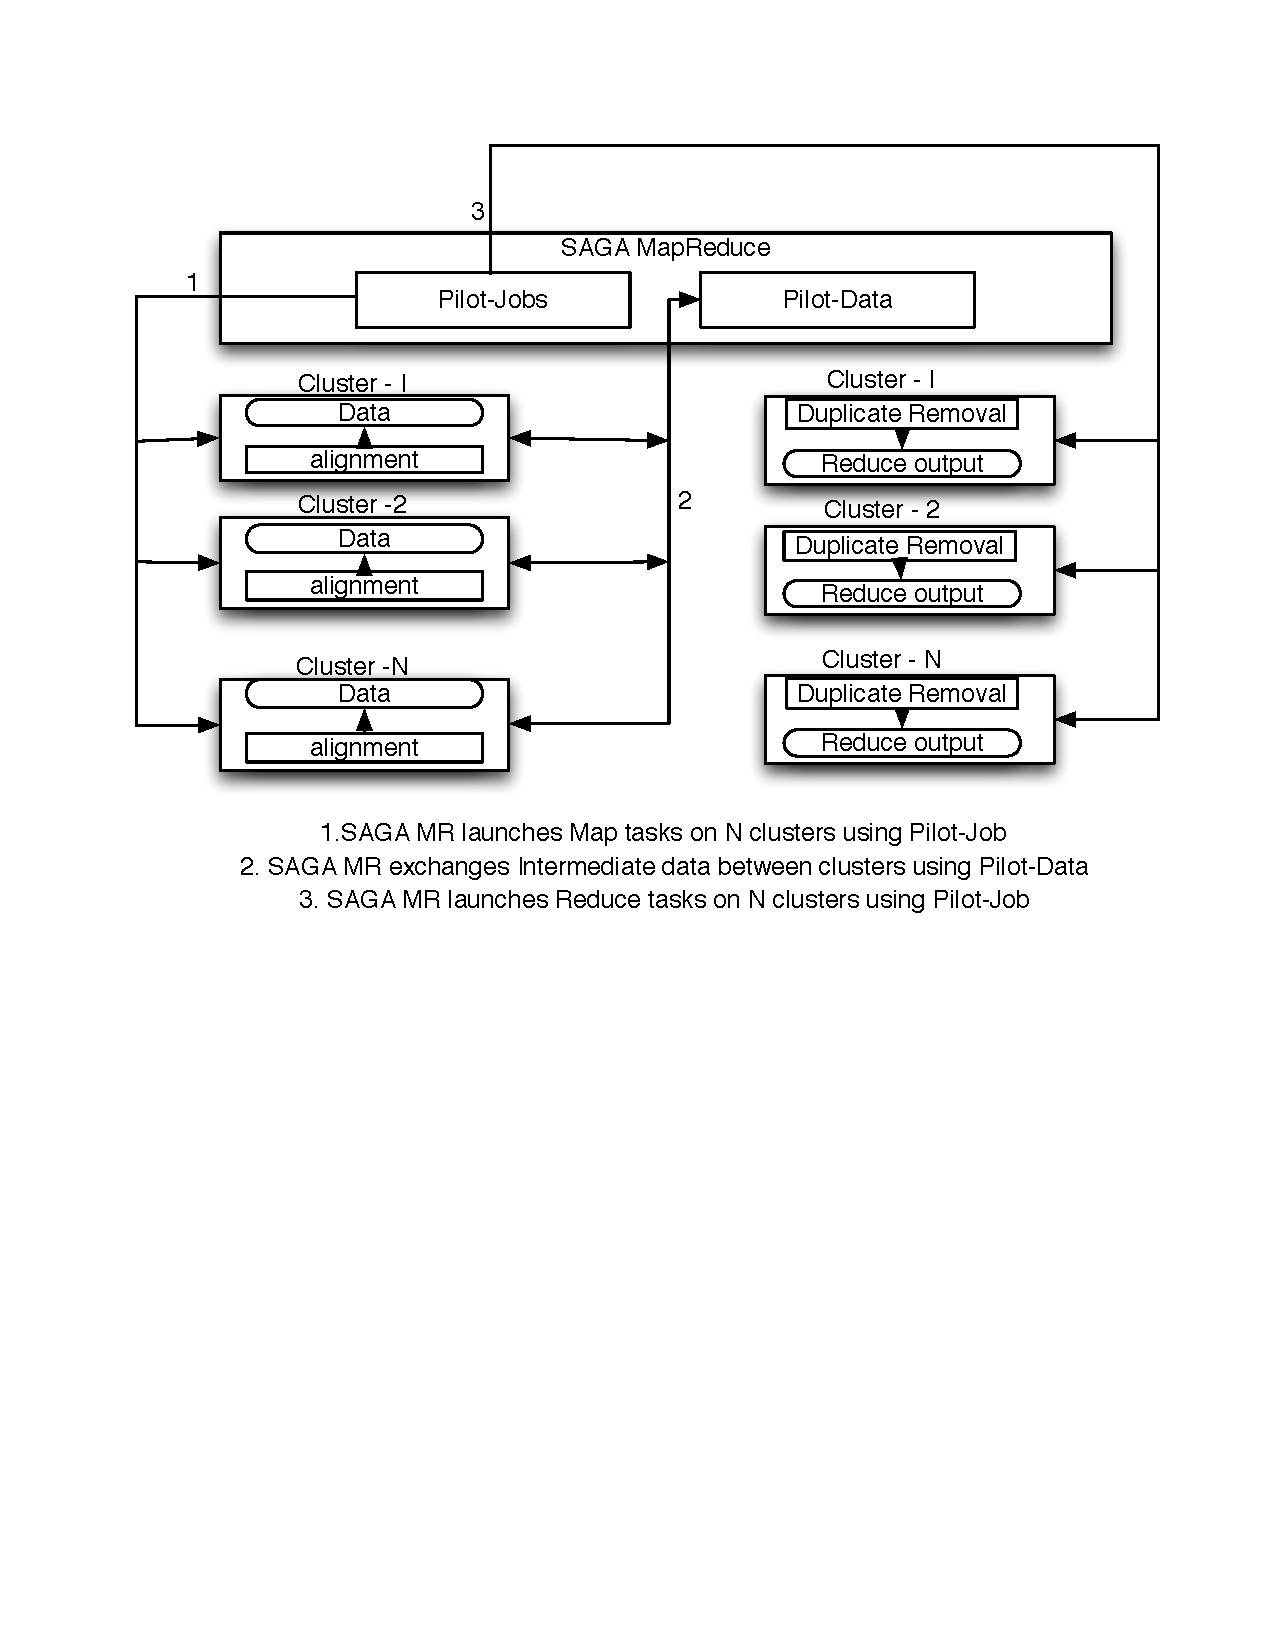
\includegraphics[scale=0.45]{figures/align-dup.pdf} 

\caption{\small Overall architecture}
  \label{fig:arch-pj-saga-mr} 
\end{figure}


\subsection{Characteristics}

There are unique features that differentiate our approach from others, which could be beneficial for developing cyberinfrastructure for NGS data analytics and downstream analysis.  
\begin{enumerate}

\item MapReduce via Parallel/Concurrency framework vs. MapReduce as a API embedded in an Application or a pipeline  
\item No need of Hadoop infrastructure
\item Scalability by utilizing multiple compute resources
\item Distributed data across distributed resources
\end{enumerate}
 
 

\begin{center}
\begin{table*}[ht]
{\small
\hfill{}
\begin{tabular}{|l|l|c|c|c|c|c|c|}
\hline
  & \textbf{SAGA-MapReduce}\cite{pj_sagamr} & \textbf{SEQAL}\cite{seal2011} & \textbf{Crossbow}\cite{langmead2009} & \textbf{CloudBurst}\cite{cloudburst} & \textbf{GATK}\cite{gatk} \\ \hline
%\cline{3-9}
 \hline 
 Key Feature & PilotJob   &  Hadoop  &  Hadoop & Hadoop & \\ 
  &   & (HDFS)  &  (HDFS) & (HDFS) & \\ \hline
Target Tasks & Alignment/Duplicate Removal & Alignment/ & Alignment/ & Alignment & \\
       &  or Alignment/Others (RNA-Seq, & Duplicate & SNP Discovery & & \\ 
        & ChIP-Seq, and Many) &  Removal & &  & \\ \hline  
Multiple  & Yes  & No  & No & No  &\\
Resources   & &  &   &  &\\  &  &  &  &  & \\ \hline

Strength & 1. Scalable with Multiple Systems  &  &  &  & \\ 

&  2. Pilot Job/Data Support & &  & & \\ 
&3. Extensibility  &  &  &  & \\
& 4. Short Development Cycle & & & & \\\hline
Weakness &  & 1. HDFS Limitations & 1. HDFS Limitations & 1. HDFS Limitations  &\\ \hline

\hline
\end{tabular}}
\hfill{}
\caption{Comparison of Next-Generation Sequencing (NGS) tools implemented with MapReduce}
 \label{table:mr-comparison}
\end{table*}
\end{center}


% \begin{table}
% \small
% \begin{tabular}{|c|c|c|c|c|} 
% \hline 
%   &  SAGA- & SEQAL & Crossbow & CloudBurst \\ 
%   & MapReduce &  &  \\\hline
% Key  & PilotJob   &  Hadoop  &  Hadoop & Hadoop \\ 
% Aspect &   & (HDFS)  &  (HDFS) & (HDFS) \\ \hline
%Target & Alignment/ & Alignment/ & Alignment/ & Alignment \\
% Tasks       & Multiple & Duplicate & SNP & \\ 
%        & Analyses &  Removal & &  \\ \hline  
%Distri-  & Fully   & Hard  & Hard & Hard \\
%buted   & interoperable &  &   & \\ 
%Resources &  &  &  & \\ \hline
%
%Strength & 1. Multiple  &  &  &  \\ 
%& Resource &  &  &  \\
%&  2. Decoupling & &  &  \\ 
%& of Map/Reduce &  &  &  \\ \hline
%Weakness &  & 1. HDFS & 1. HDFS & 1. HDFS \\ \hline
%
%\hline
%\end{tabular}
%\caption{Comparison of Next-Generation Sequencing (NGS) tools implemented with MapRedue}
%  
%  \label{table:mr-comparison} 
%\end{table}

\begin{figure}
 \centering
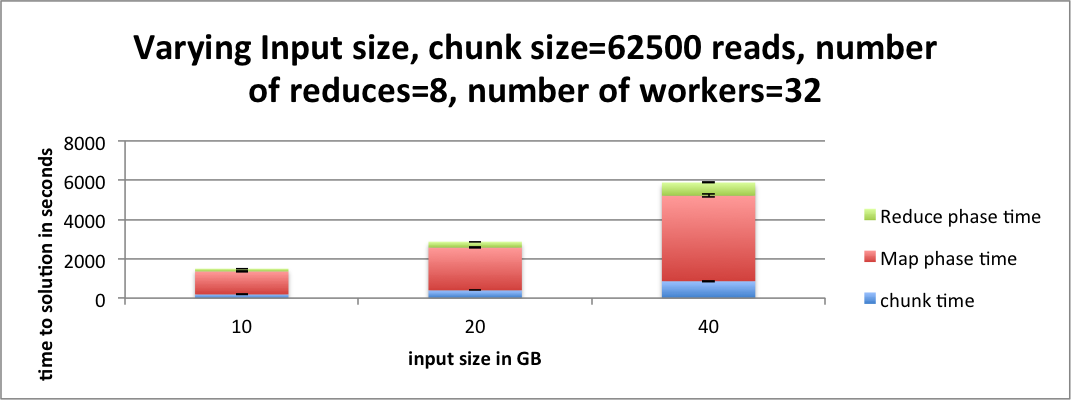
\includegraphics[scale=0.45]{figures/pj-smr-tts.png} 
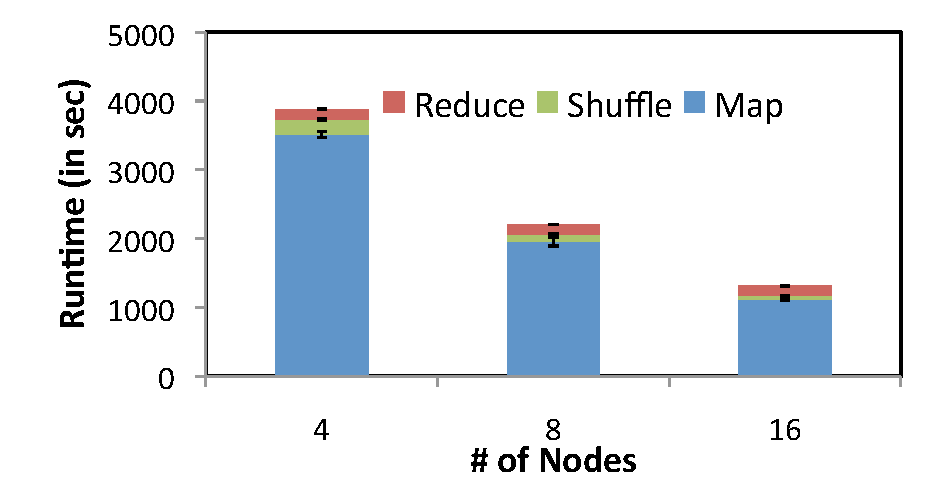
\includegraphics[scale=0.42]{figures/pj-smr-scale.pdf}


\caption{\small PJ-based SAGA-MapReduce}
  \label{fig:scale-pj-saga-mr} 
\end{figure}


\section{Performance}


\begin{figure}
 \centering
\includegraphics[scale=0.45]{} 

\caption{\small Performance comparison}
  \label{fig:comp-pj-saga-mr} 
\end{figure}

\section{Conclusion and Future Work}


% \begin{table}
% \small
% \begin{tabular}{|c|c|c|c|c|c|} 
% \hline 
%Case & Read File & Threads   &  \# of & BigJob Size   &   $T_C$   \\
%   & Size& per Task & Tasks  & Cores(Nodes)  & \\
%   \hline
%g1 & 0.209 GB & 2 &   40 &  80(10) & 3966 s \\
%g2 & 0.435 GB & 2 &  20 & 40(5) & 8031 s\\ \hline
%g3  & 0.209 GB& 2 & 40  & 12(3) & 25807 s \\
%g4 & 0.435 GB& 2 & 20  & 12(3) & 23872 s  \\ \hline
%\hline
%g5 & 0.209 GB& 2& 40 & 80(20) & 1111 s \\
%g6&0.435 GB&2& 20 & 40(10)&2096 s\\
%\hline
%\end{tabular}
%\caption{Performance comparison for different parallel configurations
%  using SAGA-BigJob on a HPC-Grid (LONI). One BigJob is submitted with
%  the number of sub-jobs, where each sub-job is a BFAST task.  The
%  total (read) data size is the read-file size multiplied by the
%  number of tasks (which is equal to the number of read-files); which
%  is a constant for g1-g6.  Cases g1, g2 and g3,g4 and g5,g6 are
%  conducted on QB, Painter and Eric respectively. The cases g1, g2,
%  g3, g4 are use 40 index files of a Human Chromosome 21.  Note that
%  g5 and g6 are the results with 10 index files; g6 is specifically
%  carried out to provide a direct comparison to c5 (on a cloud
%  resource as in the following Table~\ref{table:cloud-VM}) }
%  
%  \label{table:bigjob-loni} 
%\end{table}



\section*{Acknowledgement}
This document was developed with support from the National Science
Foundation (NSF) under Grant No.  0910812 to Indiana University for
``FutureGrid: An Experimental, High-Performance Grid Test-bed.''  We
also acknowledge Ole Weidner and Le Yan for useful performance related
discussions, Diana Holmes for sharing her experience with mapping
using BFAST, and Jong-Hyun Ham for allowing us to use B. Glumae genome
sequences.  Computing resources were made possible via NSF TRAC award
TG-MCB090174 and LONI resources.  The project described was partially
supported by Grant Number P20RR016456 from the NIH National Center For
Research Resources.

\bibliographystyle{abbrv} 
\bibliography{compbio}
\bibliography{saga}


\end{document}

Any opinions, ndings, and conclusions or recommendations expressed in
this material are those of the author(s) and do not necessarily
reflect the views.
